%% Paper 2 -- compile with:  latexmk -lualatex main.tex   (or Overleaf, compiler = LuaLaTeX)
\documentclass[preprint,12pt,authoryear,nonatbib]{elsarticle}
% APA 7 is the default. Define \APASix before inputting this file only for legacy builds.
\ifdefined\APASix\else\def\APASeven{1}\fi
\ifdefined\APASeven
  \usepackage[english]{babel}
  \usepackage{csquotes}
  \usepackage[backend=biber,style=apa,natbib=true]{biblatex}
  \addbibresource{refs.bib}
\else
  \usepackage[natbibapa]{apacite}
\fi
\usepackage{fontspec}            % Unicode (Vietnamese abstract) with LuaLaTeX/XeLaTeX
\setmainfont{Latin Modern Roman}
\usepackage{amsmath,amssymb}
\usepackage{graphicx,booktabs,tabularx,multirow,makecell,float}
\usepackage[margin=2.5cm]{geometry}
\usepackage{xcolor,enumitem,setspace}
\usepackage[hidelinks]{hyperref}
\usepackage{lineno}
\usepackage{microtype}
\setlength{\emergencystretch}{1em}
\onehalfspacing
\newcommand{\tbd}[1]{\textcolor{red}{[#1]}}   % administrative details to be supplied by the authors
\graphicspath{{figures/}}
\journal{Computers and Education: Artificial Intelligence (target) / HNUE--UNESCO International Conference 2027}

% Vietnamese abstract: keep for the HNUE conference version; set \vietnamesefalse for journal submission
\newif\ifvietnamese
\vietnamesetrue
\begin{document}
\begin{frontmatter}
\title{Locally deployed small language models on a national high-stakes examination: Benchmarking against eight years of Vietnamese candidate scores}

% Anonymous review draft. Supply verified author metadata on a separate title page.

\begin{abstract}
Generative AI challenges the security and validity of high-stakes examinations, but accuracy alone does not show how models compare with real candidates. We study Viet Nam's National High School Graduation Examination using five open sources: 1,700 official items from eight multiple-choice subjects (2019--2023); 383 presentations of 236 audited hard items; 7.29 million candidate records (2017--2024); official statistics for validation; and provincial socio-economic indicators. Three quantised open-weight models run locally through Ollama. We link their exam-score equivalents to national and provincial candidate distributions, analyse item-position and restricted-input associations, and test option-order and response-format sensitivity. Candidate means rose across the eight years, with marked ceiling effects in civic education and persistent provincial income gradients in mathematics and English. The highest overall S1 accuracy was 67.9\% (Gemma 2 (9B)). Its mean national percentile was 91.8 in English but 21.4 in mathematics, demonstrating that AI advantage is strongly subject-dependent. Qwen's hard-item MCQ--open accuracy gaps were 12.4 percentage points in chemistry and 17.2 in physics; these format effects do not by themselves establish contamination.
 A fixed model score tends to rank higher against candidates in lower-income provinces in English and mathematics. These historical, text-only comparisons provide a baseline for evaluating examination reform and support repeated audits with complete stimuli, transparent grading and secure administration.
\end{abstract}

\begin{keyword}
large language models \sep high-stakes assessment \sep national examination \sep local inference \sep assessment validity \sep educational equity \sep Viet Nam
\end{keyword}
\end{frontmatter}

\ifvietnamese
\noindent\textbf{Tóm tắt.} Trí tuệ nhân tạo tạo sinh hiện có thể trả lời nhiều câu hỏi thi chuẩn hóa. Điều này đe dọa tính hiệu lực và an ninh của các kỳ thi quan trọng, đồng thời đặt ra câu hỏi kỳ thi quốc gia nên đánh giá điều gì. Nghiên cứu kết hợp năm nguồn dữ liệu mở về kỳ thi tốt nghiệp THPT của Việt Nam: (i) 1.700 câu hỏi của 5 đề chính thức 2019--2023 thuộc 8 môn trắc nghiệm (VNHSGE); (ii) 383 lượt trình bày của 236 câu khó có đáp án số đơn kiểm tra được, với câu Toán trả lời số và câu Hóa/Lý ở cả hai dạng; (iii) 7,29 triệu bản ghi điểm thi cấp thí sinh giai đoạn 2017--2024; (iv) thống kê điểm do Bộ GDĐT công bố, dùng để kiểm định; và (v) chỉ số thu nhập và vùng dân tộc thiểu số cấp tỉnh. Nghiên cứu đánh giá ba mô hình ngôn ngữ lớn có trọng số mở, được lượng tử hóa và chạy local; xác định thứ hạng của từng mô hình trong phân phối điểm của thí sinh thật ở cấp quốc gia và cấp tỉnh; tìm các đặc điểm câu hỏi khiến AI trả lời sai; và kiểm tra hiện tượng nhiễm dữ liệu huấn luyện bằng cách xáo trộn phương án và đổi dạng câu hỏi. Dữ liệu thí sinh cho thấy điểm trung bình tăng trong tám năm khảo sát, hiệu ứng trần (tới 40\% thí sinh đạt từ 9 điểm môn GDCD), và chênh lệch theo thu nhập giữa các tỉnh ổn định ở môn Toán và Tiếng Anh. Mô hình có độ chính xác tổng thể cao nhất trên S1 là Gemma 2 (9B) (67.9\%); bách phân vị quốc gia trung bình đạt 91.8 ở môn Tiếng Anh nhưng chỉ 21.4 ở môn Toán. Trên bộ câu khó đã kiểm tra đáp án, chênh lệch trắc nghiệm--trả lời số của Qwen là 12.4 điểm phần trăm ở Hóa và 17.2 ở Lý. Các khác biệt theo dạng câu không đủ để kết luận về nhiễm dữ liệu huấn luyện.
 Nghiên cứu thảo luận hàm ý cho đổi mới kỳ thi từ năm 2025: thiết kế câu hỏi bền vững trước AI, an ninh kỳ thi trước thiết bị tích hợp AI, công bằng giữa các tỉnh, và sử dụng LLM có trách nhiệm trong rà soát đề thi.
\fi

\linenumbers
\section{Introduction}

Large language models (LLMs) now reach or exceed the level of human test-takers on many standardised examinations, from professional licensing tests to university-entrance examinations \citep{openai2023gpt4,zhang2023m3exam}. For education systems this creates two problems. The first concerns \emph{security and validity}. A model on a phone can answer exam items in seconds, so an examination that cannot exclude such devices no longer measures what it claims to measure \citep{cotton2024}. The second concerns \emph{purpose}. If routine recall items can be answered by machines, a national examination that rewards such items also signals to teachers, through ``teaching to the test'' \citep{koretz2017}, that students should spend time on what machines already do well \citep{swiecki2022,unesco2023genai}.

Viet Nam's National High School Graduation Examination is taken by about one million candidates each year and is used for both graduation and university admission. From 2017 to 2024 it consisted almost entirely of four-option multiple-choice items assembled according to a four-level cognitive matrix. From 2025 it follows the 2018 General Education Curriculum, with new item formats and an explicit emphasis on competencies \citep{moet2023plan}. The reform thus coincides with the arrival of generative AI. Earlier work introduced the VNHSGE benchmark and showed that ChatGPT approached human-level scores in language-heavy subjects but not in mathematics and the sciences \citep{dao2023vnhsge,dao2023math}. Three questions that matter for assessment policy remain open: (a) where current models stand \emph{relative to the real population of candidates}, not only relative to a national mean; (b) \emph{which recorded item characteristics} predict errors under a specified protocol; and (c) whether high accuracy reflects reasoning or \emph{memorisation} of widely published past papers.

We address these questions with a multi-source design. We extend accuracy-based benchmarking by linking item-level model performance with eight years of candidate-level score data (7.29 million records), validated against official statistics, and with provincial socio-economic indicators. This lets us express AI performance in the metric that matters to students and policy makers, namely the percentile a candidate would reach, nationally and in each province. We ask:

\begin{enumerate}[label=\textbf{RQ\arabic*.},leftmargin=*]
  \item How accurately do the three locally deployed open-weight LLMs answer the examination, and what percentile would their scores reach among real Vietnamese candidates?
  \item Which recorded item characteristics (position bands, omitted visual resources, notation and length) are associated with errors under the text-only direct-answer protocol?
  \item Are LLM answers robust to option order and to the removal of options, or do they suggest memorisation?
  \item How has the candidate score distribution evolved over 2017--2024, and how does the advantage an ``AI answer machine'' would confer differ across provinces with different socio-economic conditions?
\end{enumerate}

\section{Background}
\subsection{LLMs on human examinations}
Benchmarks built from human examinations, such as MMLU \citep{hendrycks2021mmlu}, AGIEval \citep{zhong2024agieval} and M3Exam \citep{zhang2023m3exam}, are now the standard way to compare LLMs. Performance is uneven: models do best in language-rich, recall-heavy domains and worst in multi-step quantitative reasoning and figure-dependent items. Performance in lower-resource languages lags behind English. For Vietnamese, the VNHSGE dataset compiled national examination papers with answer keys and explanations \citep{dao2023vnhsge}.

\subsection{National entrance-examination benchmarks}
Related national examinations help distinguish answering accuracy from educational interpretation. In China, GAOKAO-Bench evaluates objective and subjective questions across subjects and converts model performance to examination scores \citep{zhang2023gaokao}. GAOKAO-Eval subsequently examines recently released papers and uses Rasch analysis to question whether high scores imply human-aligned difficulty patterns \citep{lei2024gaokao}. The latter remains a preprint in the source record consulted here. These studies motivate explicit attention to item exposure and response processes, but their Chinese-language scores cannot be transferred directly to Vietnamese candidates.

In Korea, a study of the 2026 CSAT mathematics examination evaluates models shortly after the public release of the paper, comparing input modalities and prompt languages \citep{pyeon2025csat}. This preprint illustrates a practical strategy for reducing exposure to the particular examination before testing. Freshness alone does not equate machine and human ability, and neither model rankings nor modality effects should be assumed constant across examination systems. Our retrospective S1 design provides a longer historical reference but offers weaker control over item exposure.

Brazil's ENEM supplies a particularly relevant comparison for local inference: quantised LLaMA-based models were evaluated on Portuguese and translated English items using consumer hardware \citep{santos2023enem}. Subsequent ENEM word-problem research separates textual interpretation from equation solving, showing that these demands can produce different model performance patterns \citep{calais2025}. A 2026 preprint additionally benchmarks estimated difficulty against official ENEM IRT parameters \citep{brant2026enem}. These approaches distinguish three targets---answering items, modelling their demands and reproducing human difficulty---that should not be conflated. Our contribution is the linkage of observed model scores to national and provincial candidate distributions, while item-response calibration remains unavailable for S3.

\subsection{Robustness and contamination}
Multiple-choice accuracy may overstate competence. LLMs are sensitive to option order and favour particular option letters \citep{pezeshkpour2024,zheng2024mcq}. Past national papers and their keys are widely published online and may have been included in training data, so a model may \emph{recognise} rather than \emph{solve} items. Contamination is commonly probed by comparing performance on original and perturbed versions of the same item \citep{golchin2025}. We use two perturbations: shuffling the options, which leaves difficulty unchanged for humans, and removing the options so that the value must be produced (open format).

\subsection{Assessment in the age of AI}
Scholars argue that generative AI makes assessments that reward the reproduction of information obsolete. They call for authentic, process-oriented assessment and for explicit rules on permitted AI use \citep{swiecki2022,perkins2024aias}, while recognising that LLMs can also support item writing and feedback \citep{kasneci2023}. Most of this work concerns coursework in higher education. Evidence on invigilated national examinations in middle-income systems, which still determine life chances and shape teaching, is scarce. Item demand in the Vietnamese papers follows a four-level matrix adapted from the revised Bloom taxonomy \citep{anderson2001}: recognition, comprehension, application and high-level application.

Recent reviews broaden this discussion beyond whether an answer is correct. A scoping review identifies replicability, transparency, privacy and equality as central challenges for educational LLM applications \citep{yan2024}; another organises assessment implications at student, teacher and institutional levels \citep{xia2024assessment}. From an educational-measurement perspective, deploying generative models raises questions about reliability, fairness and test security alongside efficiency \citep{hao2024}. Work on validity and evaluative judgement further argues for evidence about the knowledge demonstrated and the learner's ability to judge the quality of AI outputs \citep{kaldaras2024,bearman2024}. These concerns inform our separation of candidate-relative ranks from claims about competence or actual gains from assistance.

\subsection{Security and ethical safeguards}
Empirical studies make clear that assessment design and detection are separate issues. AI-written submissions entered an unsupervised university examination system with many going undetected \citep{scarfe2024}; a study in two UK business schools also investigates the academic-integrity implications for authentic assessments \citep{kofinas2025}. Neither setting estimates cheating prevalence in an invigilated national examination. Teacher judgements of essay authorship and software detection also have documented limitations \citep{fleckenstein2024,weberwulff2023}, with evidence of unequal false-positive risks for non-native English writers \citep{liang2023}. These writing studies do not validate detection of AI-assisted multiple-choice responses and therefore cannot justify automatic accusations based on this benchmark.

For large-scale examinations, safeguards must address the entire testing process. International Test Commission guidelines cover security planning, administration and responses to breaches \citep{itc2014security}; the educational and psychological testing standards connect defensible score use with validity and fairness \citep{aera2014}. Applied here, a model-capability audit is one source of evidence for planning controls on unauthorised assistance and item exposure, rather than a replacement for invigilation or incident investigation. A responsible policy also distinguishes prohibited examination assistance from legitimate learning support, specifies permitted resources and retains human review of consequential decisions. This combination connects the international literature to the present local-model and provincial-distribution design.

\subsection{Interpretation and use of model scores}
Kane's argument-based framework distinguishes scoring, generalisation, extrapolation and the justification of score uses \citep{kane2013}. Here, answer-key grading supports a scoring inference for the observed model responses. Generalisation is limited to the sampled papers, model binaries, quantisation and prompts. Extrapolation from correct answers to the intended student competence is not established: a machine may produce the same answer through a different process, and withheld stimuli change the task. Candidate percentiles provide a historical reference distribution, not evidence of equivalent latent ability. The decision inference concerning graduation or admission would require evidence about permitted assistance, secure administration and consequences; this benchmark does not supply that evidence. We therefore treat AI resilience as conditional on the model, input access and administration conditions, rather than an intrinsic property established by low model accuracy.

An item-response framework would additionally distinguish difficulty, discrimination and lower-asymptote parameters \citep{lord1974}. The theoretical four-option guessing probability is 0.25, but it is not an estimated item-specific IRT parameter. S3 contains total subject scores, not candidate item responses; it cannot identify item difficulties, calibrate an IRT model, or test differential item functioning between humans and models. Provincial rank differences are distributional comparisons, not DIF. The position bands are exploratory descriptors and must not substitute for those psychometric quantities. Multimodal benchmarks such as MathVista further show why complete visual stimuli are necessary when studying mathematical competence \citep{lu2024mathvista}.

\section{Data}
Table~\ref{tab:sources} summarises the five open data sources. All are publicly downloadable without registration; the code and download scripts are provided (Section~\ref{sec:availability}).

\begin{table}[H]\centering\small
\caption{Data sources}\label{tab:sources}
\begin{tabularx}{\textwidth}{@{}l>{\raggedright}p{3.8cm}X@{}}
\toprule
\# & Source & Content and use\\
\midrule
S1 & VNHSGE evaluation set \citep{dao2023vnhsge} & Official 2019--2023 papers, 8 MCQ subjects, 1,700 items with keys and images. LLM benchmark (RQ1--RQ3).\\
 S2 & Vietnamese Entrance Exam \citep{iithought2025} & Audited scalar-answer subset: 89 mathematics items with paper year (2017--2024); 89 chemistry and 58 physics items with options, each shown twice. MCQ vs open format; exploratory year comparison (RQ3).\\
S3 & Candidate-level scores 2017--2024 \citep{thptqgscores} & 7,287,744 records (registration number, province, subject scores; no names). Human benchmark and provincial analysis (RQ1, RQ4).\\
S4 & MOET published score statistics \citep{moet2023scores} & National means by subject and year. Validation of S3.\\
S5 & Provincial indicators \citep{odm2018income,odm2015ethnic} & Income per capita 2018 (GSO/VHLSS) and population of ethnic-minority areas 2015, 63 provinces. Equity analysis (RQ4).\\
\bottomrule
\end{tabularx}
\end{table}

\paragraph{Item banks} Table~\ref{tab:itembank} describes S1. Ninety-seven items require an image (mostly mathematics and physics). Sixty-eight geography items (34\%) require the printed \emph{Atlat Địa lí Việt Nam}, which candidates bring into the examination room but which is not part of the item. We use these items as an ``external resource omitted'' condition. Answer keys over-represent option A (29.9\%), so we also report models' answer-letter distributions. S2 is a curated difficult-item dataset, with some stems reformulated by its provider; it is not a second representative sample of complete examination papers. Of the 432 source records, we retain 236 Vietnamese items whose released answers are complete decimal scalars and, for chemistry and physics, have exactly one numerically matching option. Symbolic expressions, fractions, multi-value answers and items without an unambiguous option match are excluded rather than reduced to their first number. The resulting 383 presentations comprise 89 mathematics items in open format, and 89 chemistry plus 58 physics items each shown with and without options (Table~\ref{tab:hard}). Mathematics years come from source labels; chemistry and physics years are unavailable. An exclusion log accompanies the code. This conservative restriction makes numerical grading reproducible but limits generalisation to other hard-item answer types.

\begin{table}[H]\centering\small
\caption{S1 item bank: official examinations 2019--2023}\label{tab:itembank}
\begin{tabular}{@{}lrrrrrr@{}}
\toprule
Subject & Items & Items/paper & Image & Atlas & LaTeX & Mean length (chars) \\
\midrule
Mathematics & 250 & 50 & 53 & -- & 104 & 192 \\
Physics & 200 & 40 & 20 & -- & 19 & 295 \\
Chemistry & 200 & 40 & 4 & -- & 159 & 267 \\
Biology & 200 & 40 & 10 & -- & 0 & 305 \\
History & 200 & 40 & 0 & -- & 0 & 278 \\
Geography & 200 & 40 & 10 & 68 & 0 & 236 \\
Civic education & 200 & 40 & 0 & -- & 1 & 321 \\
English & 250 & 50 & 0 & -- & 0 & 862 \\
\midrule
Total & 1,700 & & 97 & 68 & 283 & \\
\bottomrule
\end{tabular}

\par\smallskip\raggedright\footnotesize\textit{Note.} LaTeX counts items containing formula markup; it indicates notation presence, not a validated measure of mathematical or chemical complexity. Image and atlas counts identify resources omitted from model inputs.
\end{table}

\begin{table}[H]\centering\small
\caption{S2 hard item set (presentations by format)}\label{tab:hard}
\begin{tabular}{@{}lrr@{}}
\toprule
Subject & MCQ & Open \\
\midrule
Chemistry & 89 & 89 \\
Mathematics & 0 & 89 \\
Physics & 58 & 58 \\
\bottomrule
\end{tabular}

\end{table}

\paragraph{Candidate scores and validation} S3 is a third-party mirror of publicly accessible examination results. The repository's documentation and accompanying crawler artifacts identify Vietnamese news-media results portals, including Dan Tri (the documented 2022 collector) and VietNamNet (the accompanying 2021 notebook), as collection sources \citep{thptqgscores}. We cross-check the mirrored scores against MOET's published national means as an aggregate data-integrity check (Table~\ref{tab:validation}). These artifacts document collection routes but do not provide a complete per-year lineage for all eight CSV files; agreement of means does not certify completeness or the integrity of every record. It contains each candidate's registration number, province code and subject scores, without names; we analyse only aggregates. Coverage is incomplete in three years: in 2017 records for Ha Noi and Ho Chi Minh City are capped at 64,999; 2018 covers 59 provinces (Son La missing; Ha Noi and Ha Giang partial); and 2019 lacks Ho Chi Minh City. National means nevertheless reproduce MOET's published means to within $\pm0.02$ points in 27 of 29 subject-years with published values; the largest deviations are $-0.12$ (English 2019) and $-0.07$ (mathematics 2019), where Ho Chi Minh City is missing (Table~\ref{tab:validation} in the Appendix).

\section{Method}
\subsection{Models and procedure}
We evaluate three open-weight instruction models, Qwen2.5-7B, Llama-3.1-8B and Gemma-2-9B \citep{qwen2025,llama2024,gemma2024}, and a seeded random-guessing baseline. The models run locally through Ollama with four-bit quantisation (Q4\_K\_M for Qwen and Llama; Q4\_0 for Gemma). The continuation used a 4,096-token runtime context; the model manifest records full local digests and Ollama version. Digests were not logged with the legacy responses, so their exact binary provenance cannot be independently established. Initial S1 responses were collected on an RTX 3050 with 6\,GB VRAM; the remaining Gemma responses and the S2 experiment were completed on an RTX 5060 Ti with 16\,GB VRAM in October 2026. The study evaluates these specific model versions, rather than frontier AI capability in general. Each S1 item was presented in Vietnamese with a fixed system prompt, temperature 0 and a maximum of eight output tokens, requesting a single answer letter. Qwen2.5-7B was additionally evaluated on S2 with a brief step-by-step reasoning prompt and a final answer line (up to 900 output tokens). No images or atlas pages were supplied, so all results concern text-only access to the released item content. The image and atlas conditions are information-deprivation conditions; they do not estimate multimodal performance. The eight-token direct-answer cap provides no scratchpad and can disadvantage quantitative reasoning. Because S2 changes both the item sample and the prompting protocol, S1--S2 contrasts cannot estimate the causal effect of reasoning prompts. Single-pass temperature-zero decoding also does not quantify run-to-run or backend variability; Wilson intervals are not decoding-repeat confidence intervals. Open-format answers were graded numerically with a 1\% relative tolerance plus $10^{-6}$ absolute tolerance; unparseable answers counted as incorrect. Raw responses, token counts and latencies were logged. The baseline uses a fixed pseudo-random seed and is a realised draw rather than the theoretical 25\% chance rate.

\subsection{Cognitive level, item features and contamination probes}
We assign an exploratory position-based proxy from each S1 item's relative position, using a 40/30/20/10 split to approximate recognition, comprehension, application and high-level application. This assumes that later items generally impose greater demand; it is not an expert-coded Bloom classification. Independent teacher validation has not been conducted, and no inter-rater reliability coefficient is available. For each model we fit a logistic regression of correctness on this proxy, image dependence, LaTeX notation, $\log$(item length) and subject fixed effects. These associations are descriptive rather than causal. For RQ3, every S1 item was presented a second time, attempting to permute its options using an item-specific seed. Seventeen option sets could not be parsed safely and retained their original order; 62 seeded permutations were the identity. We report the full paired comparison and a sensitivity analysis restricted to the 1,621 actually changed presentations. Paired accuracy was compared with McNemar's exact test \citep{mcnemar1947}. The S2 chemistry and physics items were presented in both MCQ and open format; mathematics was analysed by recorded paper year (2017--2024). Option-order robustness and format sensitivity probe response behaviour but cannot establish whether an item appeared in training data. The year analysis is exploratory because neither exposure histories nor matched item difficulty across years are known.

\subsection{Placing models among candidates}
Each paper weights items equally, so a model's exam-score equivalent is $10\times$ its proportion correct. Using S3, we compute for every subject-year the percentage of candidates scoring strictly below each score on a 0.05 grid (the national percentile), and the same percentage within each province with at least 300 valid subject scores. Tied candidate scores are excluded from the percentage below. Subject-level summaries average the five paper-year percentiles, rather than pooling different examinations into one distribution. The provincial summary describes province--subject--year comparisons, rather than the percentage of distinct provinces. We relate provincial percentiles to income (S5) using descriptive correlations. Accuracies are reported with Wilson intervals \citep{wilson1927}; these quantify item-level binomial uncertainty and do not account for common paper or stimulus dependence.

\subsection{Eight years of candidate scores}
For RQ4 we describe the score distributions by subject and year (mean, deciles, share of scores $\geq 9$), compute the spread of provincial means between provinces, and estimate the income gradient of provincial means each year with a weighted regression (weights = number of candidates; HC1 errors): provincial mean on $\log$ income, controlling for the ethnic-minority-area population share.

\section{Results}
\subsection{Eight years of candidate performance (S3--S5)}
Table~\ref{tab:decade} and Figure~\ref{fig:decade} summarise 7.29 million candidate records. Mean scores rose in every subject between 2017 and 2024, most in history (4.60 to 6.57) and literature (5.50 to 7.23). Mathematics rose from 5.18 to a peak of 6.66 in 2020 and settled at 6.45. The share of top scores varied strongly with the paper: in civic education 13.0\% of candidates scored at least 9 in 2017, 40.0\% in 2021 and 27.1\% in 2024. This ceiling limits the examination's ability to discriminate among strong candidates. Differences between provinces were large and closely tied to income in the two compulsory MCQ subjects (Table~\ref{tab:inequality}, Figure~\ref{fig:gradient}). Each log-unit of provincial income was associated with 0.67--0.98 points in mathematics and 1.16--1.67 points in English, and income and ethnic-minority-area share explained 55--67\% and 64--77\% of the provincial variance respectively, in every year. The mathematics gradient narrowed slightly (0.98 in 2017; 0.72 in 2024), whereas the English gradient did not. In the elective science subjects, the income gradient disappeared after 2020, a pattern that could reflect candidate selection into subject combinations, although this explanation cannot be tested with the available covariates.

\begin{table}[H]\centering\footnotesize
\caption{Candidate scores by subject, 2017--2024 (S3)}\label{tab:decade}
\begin{tabular}{@{}lrrrrrrrr@{}}
\toprule
Subject & 2017 & 2018 & 2019 & 2020 & 2021 & 2022 & 2023 & 2024 \\
\midrule
\multicolumn{9}{@{}l}{\emph{Mean score}} \\
Mathematics & 5.18 & 4.88 & 5.57 & 6.66 & 6.62 & 6.47 & 6.25 & 6.45 \\
Physics & 5.35 & 4.96 & 5.56 & 6.72 & 6.58 & 6.72 & 6.57 & 6.67 \\
Chemistry & 5.33 & 4.86 & 5.34 & 6.71 & 6.63 & 6.70 & 6.75 & 6.68 \\
Biology & 4.76 & 4.56 & 4.67 & 5.59 & 5.52 & 5.02 & 6.39 & 6.28 \\
History & 4.60 & 3.81 & 4.29 & 5.18 & 4.98 & 6.34 & 6.03 & 6.57 \\
Geography & 6.26 & 5.48 & 5.99 & 6.77 & 6.96 & 6.68 & 6.15 & 7.19 \\
Civic education & 7.79 & 7.16 & 7.35 & 8.12 & 8.38 & 8.03 & 8.29 & 8.16 \\
English & 4.45 & 3.93 & 4.24 & 4.57 & 5.86 & 5.16 & 5.46 & 5.51 \\
Literature & 5.50 & 5.44 & 5.44 & 6.60 & 6.48 & 6.51 & 6.86 & 7.23 \\
\addlinespace
\multicolumn{9}{@{}l}{\emph{Share of candidates scoring $\geq 9$ (\%)}} \\
Mathematics & 2.5 & 0.1 & 1.1 & 7.5 & 4.0 & 2.2 & 1.0 & 1.1 \\
Physics & 1.5 & 0.1 & 0.5 & 2.5 & 1.4 & 4.4 & 3.0 & 4.3 \\
Chemistry & 4.2 & 0.3 & 0.3 & 5.0 & 3.2 & 4.8 & 3.4 & 7.6 \\
Biology & 1.6 & 0.1 & 0.4 & 1.4 & 2.0 & 0.7 & 1.7 & 1.1 \\
History & 0.9 & 0.1 & 0.6 & 2.2 & 1.8 & 4.7 & 3.1 & 5.8 \\
Geography & 3.1 & 0.4 & 0.7 & 1.9 & 3.9 & 2.6 & 0.9 & 9.2 \\
Civic education & 13.0 & 6.0 & 9.9 & 26.4 & 40.0 & 22.4 & 35.5 & 27.1 \\
English & 2.9 & 0.6 & 1.6 & 1.7 & 12.0 & 4.0 & 5.4 & 4.3 \\
Literature & 0.3 & 0.2 & 0.1 & 1.2 & 1.6 & 2.5 & 4.3 & 8.8 \\
\addlinespace
\multicolumn{9}{@{}l}{\emph{Number of candidates}} \\
Mathematics & 829,605 & 741,024 & 807,762 & 866,581 & 924,651 & 982,670 & 1,003,373 & 1,045,613 \\
Physics & 395,874 & 323,353 & 292,166 & 293,287 & 326,085 & 325,510 & 327,189 & 345,615 \\
Chemistry & 398,089 & 326,981 & 295,544 & 295,536 & 327,670 & 327,353 & 328,118 & 346,518 \\
Biology & 384,653 & 319,605 & 291,199 & 290,377 & 322,472 & 322,185 & 324,625 & 342,378 \\
History & 497,458 & 446,118 & 542,729 & 568,581 & 601,017 & 659,617 & 683,447 & 706,214 \\
Geography & 483,337 & 433,221 & 535,897 & 555,072 & 595,451 & 657,377 & 682,134 & 704,682 \\
Civic education & 421,206 & 379,034 & 470,905 & 482,980 & 504,137 & 554,316 & 565,452 & 583,609 \\
English & 727,024 & 659,998 & 728,513 & 772,098 & 820,406 & 870,571 & 880,997 & 906,538 \\
Literature & 809,892 & 728,309 & 799,208 & 856,565 & 921,941 & 981,351 & 1,008,239 & 1,050,101 \\
\bottomrule
\end{tabular}

\end{table}

\begin{figure}[H]\centering
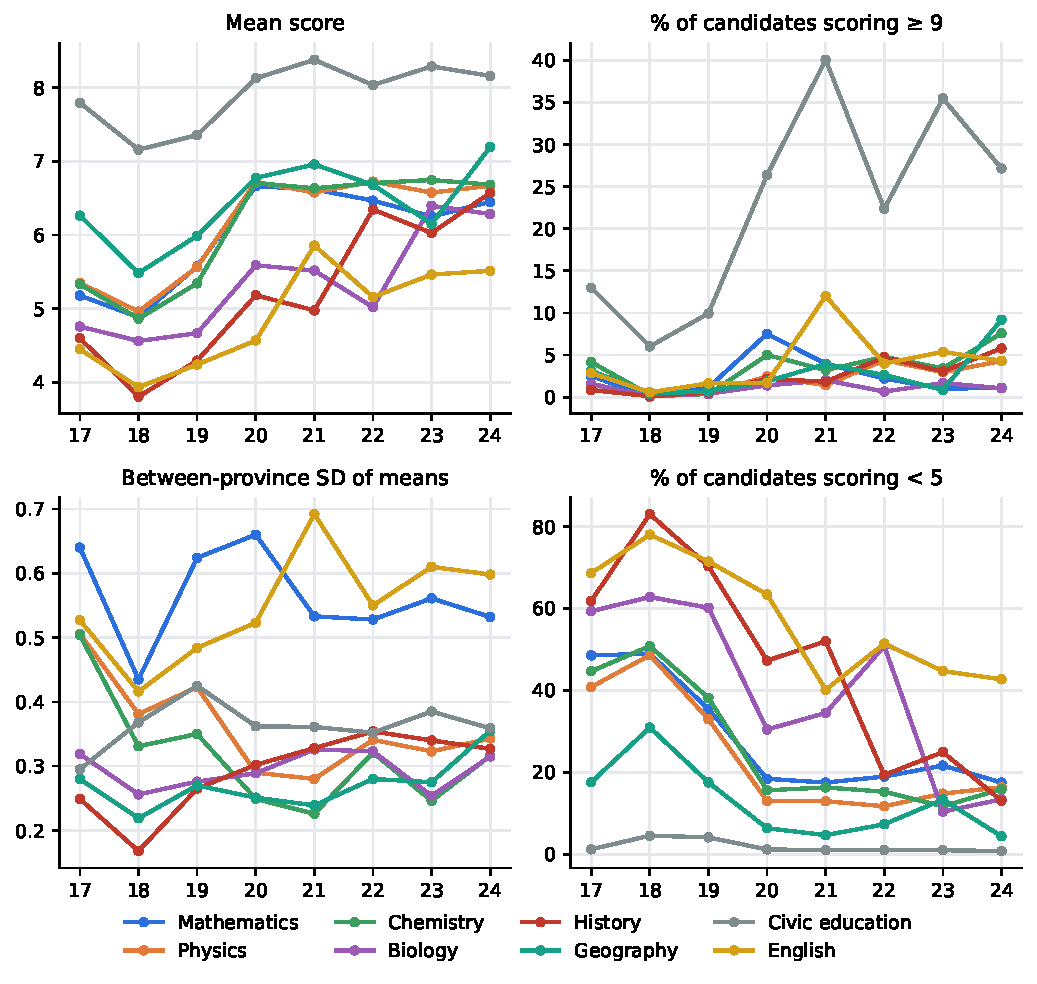
\includegraphics[width=\textwidth]{FigD1_decade_distributions.pdf}
\caption{Candidate score distributions 2017--2024: mean, share of scores $\geq 9$, spread of provincial means, and share of scores below 5.}\label{fig:decade}
\end{figure}

\begin{table}[H]\centering\footnotesize
\caption{Income gradient of provincial mean scores (points per log-unit of income; SE in parentheses below coefficients) and $R^2$ of the provincial model}\label{tab:inequality}
\begin{tabular}{@{}lrrrrrrrr@{}}
\toprule
 & 2017 & 2018 & 2019 & 2020 & 2021 & 2022 & 2023 & 2024 \\
\midrule
Mathematics & \makecell[r]{0.98 \\ (0.18)} & \makecell[r]{0.82 \\ (0.10)} & \makecell[r]{0.86 \\ (0.21)} & \makecell[r]{0.93 \\ (0.19)} & \makecell[r]{0.72 \\ (0.14)} & \makecell[r]{0.67 \\ (0.15)} & \makecell[r]{0.81 \\ (0.15)} & \makecell[r]{0.72 \\ (0.14)} \\
\quad $R^2$ & 0.61 & 0.67 & 0.55 & 0.61 & 0.61 & 0.59 & 0.63 & 0.59 \\
English & \makecell[r]{1.47 \\ (0.32)} & \makecell[r]{1.50 \\ (0.25)} & \makecell[r]{1.16 \\ (0.15)} & \makecell[r]{1.46 \\ (0.25)} & \makecell[r]{1.67 \\ (0.27)} & \makecell[r]{1.49 \\ (0.22)} & \makecell[r]{1.67 \\ (0.21)} & \makecell[r]{1.52 \\ (0.21)} \\
\quad $R^2$ & 0.67 & 0.76 & 0.64 & 0.72 & 0.74 & 0.75 & 0.77 & 0.73 \\
Physics & \makecell[r]{0.37 \\ (0.13)} & \makecell[r]{0.28 \\ (0.10)} & \makecell[r]{0.28 \\ (0.13)} & \makecell[r]{0.03 \\ (0.16)} & \makecell[r]{-0.19 \\ (0.22)} & \makecell[r]{-0.22 \\ (0.19)} & \makecell[r]{-0.08 \\ (0.21)} & \makecell[r]{-0.19 \\ (0.23)} \\
\quad $R^2$ & 0.26 & 0.21 & 0.24 & 0.10 & 0.06 & 0.04 & 0.01 & 0.04 \\
History & \makecell[r]{-0.12 \\ (0.14)} & \makecell[r]{-0.05 \\ (0.06)} & \makecell[r]{-0.01 \\ (0.12)} & \makecell[r]{0.08 \\ (0.10)} & \makecell[r]{-0.02 \\ (0.13)} & \makecell[r]{0.02 \\ (0.10)} & \makecell[r]{-0.09 \\ (0.13)} & \makecell[r]{0.03 \\ (0.09)} \\
\quad $R^2$ & 0.05 & 0.08 & 0.14 & 0.26 & 0.16 & 0.13 & 0.10 & 0.10 \\
\bottomrule
\end{tabular}

\end{table}

\begin{figure}[H]\centering
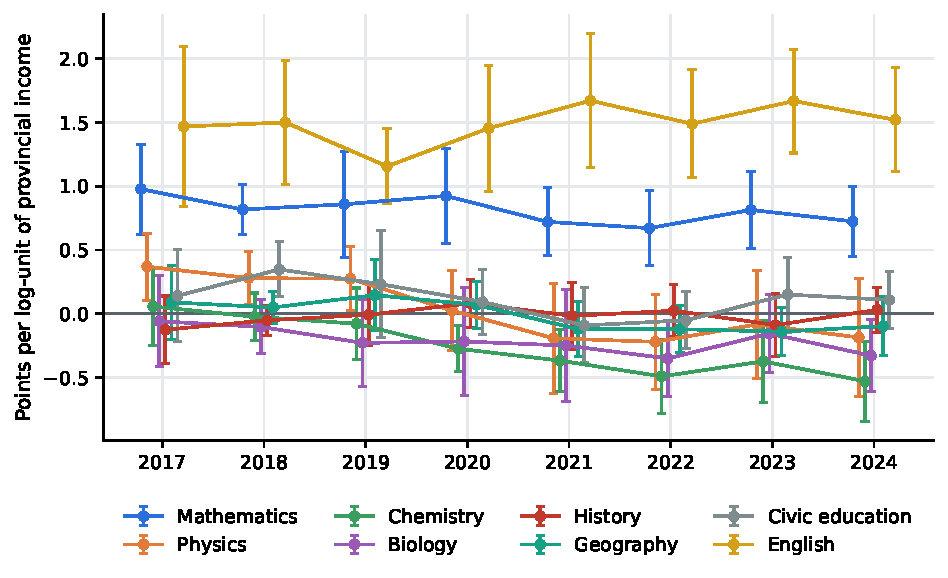
\includegraphics[width=.95\textwidth]{FigD2_income_gradient.pdf}
\caption{Income gradient of provincial mean scores by subject and year (95\% CI).}\label{fig:gradient}
\end{figure}

\subsection{LLM accuracy and percentile among candidates (RQ1)}
All three models completed both S1 conditions (1,700 items each). Overall accuracy in original option order was Gemma 2 (9B): 67.9\% (95\% CI 65.6--70.1\%); Qwen 2.5 (7B): 64.1\% (95\% CI 61.8--66.4\%); Llama 3.1 (8B): 53.9\% (95\% CI 51.6--56.3\%). The realised random baseline achieved 23.6\%, compared with the theoretical chance rate of 25\%. Table~\ref{tab:llmacc} and Figure~\ref{fig:heat} show substantial subject variation. For Gemma 2 (9B), accuracy was 86.4\% in English, 80.0\% in civic education, and 48.8\% in mathematics.

Candidate-relative performance differs from the accuracy ranking (Table~\ref{tab:llmpct}). For Gemma 2 (9B), the mean national percentile across the five paper years was 91.8 in English, 81.9 in history, 41.1 in civic education and 21.4 in mathematics. Differences in candidate distributions alter the interpretation of accuracy, especially in civic education where candidate scores cluster near the ceiling. These are averages of year-specific ranks, not a percentile for a pooled candidate population. Figure~\ref{fig:llmnat} reports the corresponding model scores against each year's national mean.


\begin{table}[H]\centering\footnotesize
\caption{Accuracy (\%) by model and subject, S1 (1,700 items, original option order, direct answers)}\label{tab:llmacc}
\begin{tabular}{@{}lrrrrrrrrr@{}}
\toprule
Model & Math & Phys & Chem & Bio & Hist & Geo & Civic & Eng & Overall \\
\midrule
Gemma 2 (9B) & 48.8 & 59.0 & 62.5 & 71.0 & 74.5 & 61.0 & 80.0 & 86.4 & 67.9 \\
Qwen 2.5 (7B) & 49.6 & 53.5 & 55.5 & 60.0 & 66.5 & 65.5 & 76.5 & 84.4 & 64.1 \\
Llama 3.1 (8B) & 29.6 & 43.5 & 48.5 & 49.5 & 63.0 & 60.0 & 76.5 & 64.4 & 53.9 \\
Random guessing & 18.8 & 28.0 & 25.0 & 26.5 & 21.0 & 23.5 & 23.0 & 24.0 & 23.6 \\
\bottomrule
\end{tabular}

\end{table}

\begin{figure}[H]\centering
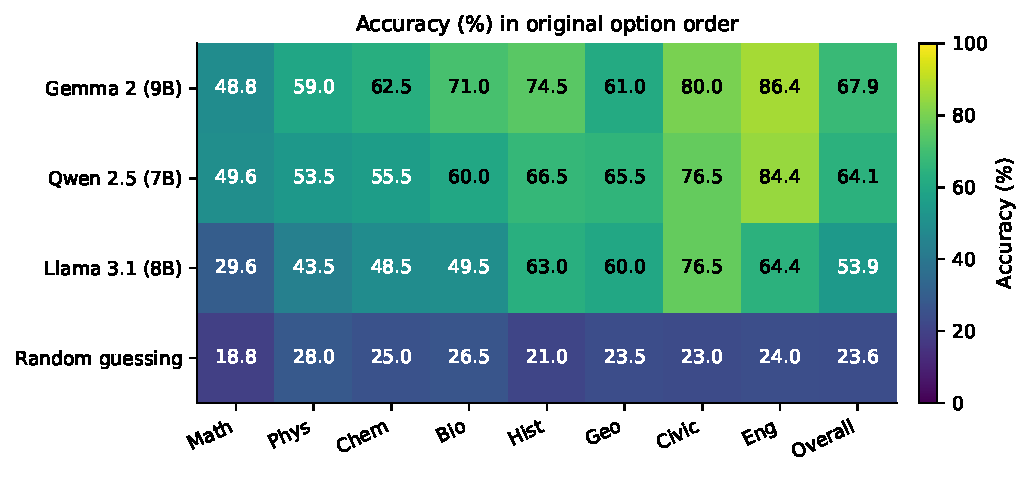
\includegraphics[width=.95\textwidth]{F1_heatmap_accuracy.pdf}
\caption{Accuracy by model and subject.}\label{fig:heat}
\end{figure}

\begin{table}[H]\centering\footnotesize
\caption{Mean national percentile of each model's exam-score equivalent (five paper years, 2019--2023), and mean share of province--year comparisons above the 50th percentile across eight subjects}\label{tab:llmpct}
\begin{tabular}{@{}lrrrrrrrrr@{}}
\toprule
Model & Math & Phys & Chem & Bio & Hist & Geo & Civic & Eng & Prov.\,$>$\,median (\%) \\
\midrule
Gemma 2 (9B) & 21.4 & 32.5 & 39.3 & 85.5 & 81.9 & 33.5 & 41.1 & 91.8 & 50.0 \\
Qwen 2.5 (7B) & 22.3 & 22.4 & 27.1 & 61.2 & 74.9 & 45.4 & 30.3 & 91.5 & 40.0 \\
Llama 3.1 (8B) & 4.5 & 9.7 & 19.2 & 34.1 & 64.6 & 33.1 & 32.5 & 73.3 & 29.3 \\
Random guessing & 0.4 & 2.2 & 0.9 & 1.1 & 1.4 & 0.2 & 0.1 & 5.5 & 0.0 \\
\bottomrule
\end{tabular}

\end{table}

\begin{figure}[H]\centering
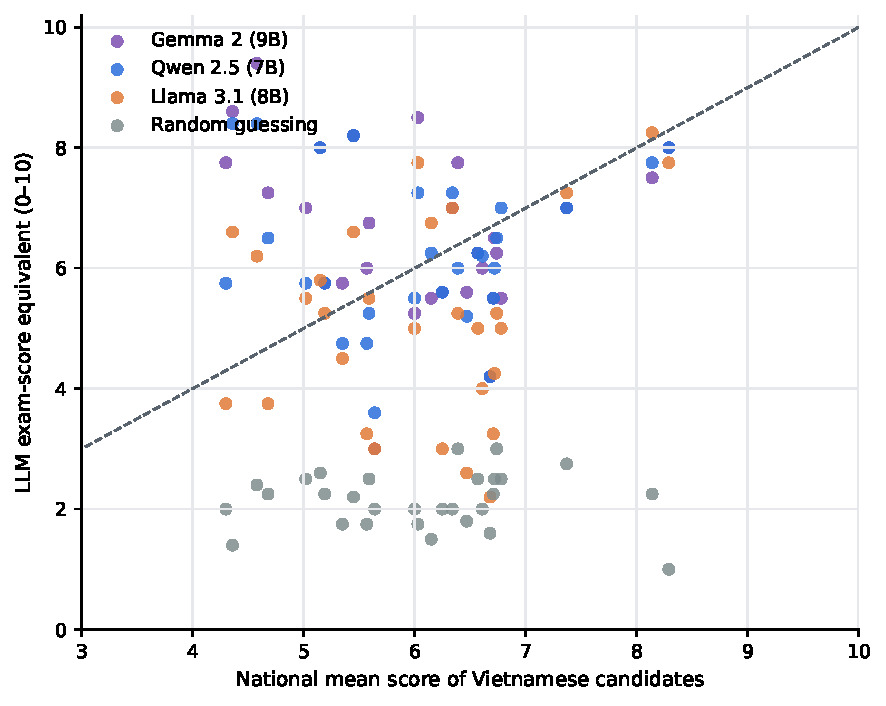
\includegraphics[width=.85\textwidth]{F3_llm_vs_national.pdf}
\caption{LLM exam-score equivalent vs the national mean of candidates, by subject and year.}\label{fig:llmnat}
\end{figure}

\subsection{Item-feature associations under restricted input access (RQ2)}
Accuracy was lower in later position bands: Gemma 2 (9B) from 76.3\% in the first position band to 51.2\% in the last; Qwen 2.5 (7B) from 72.1\% in the first position band to 44.7\% in the last; Llama 3.1 (8B) from 61.9\% in the first position band to 42.9\% in the last (Table~\ref{tab:llmlevel}, Figure~\ref{fig:level}). For Gemma 2 (9B), the adjusted odds ratio for the final band relative to the first was 0.30 (95\% CI 0.20--0.47; $p<0.001$), controlling for subject and the recorded item features. This is an association with item position; without independent cognitive coding or candidate item responses it does not validate a Bloom-level or empirical-difficulty gradient.

For Gemma 2 (9B), accuracy was 28.9\% on the 97 image-dependent items and 71.1\% on items classified as text, versus 61.8\% on the 68 atlas-dependent geography items. The image condition measures performance with required information withheld, confounding input access with model capability; its accuracy cannot establish resistance to multimodal AI, and atlas success could reflect general geographic knowledge, inference or prior exposure. The 12 table/chart items form too small a group for strong conclusions.


\begin{table}[H]\centering\footnotesize
\caption{Accuracy (\%) by unvalidated position proxy and item type}\label{tab:llmlevel}
\begin{tabular}{@{}lrrrrrrrr@{}}
\toprule
 & \multicolumn{4}{c}{Cognitive level (position proxy)} & \multicolumn{4}{c}{Item type} \\
Model & R & C & A & AA & Text & Table/chart & Image & Atlas \\
\midrule
Gemma 2 (9B) & 76.3 & 70.2 & 55.9 & 51.2 & 71.1 & 8.3 & 28.9 & 61.8 \\
Qwen 2.5 (7B) & 72.1 & 66.9 & 53.8 & 44.7 & 66.5 & 33.3 & 33.0 & 60.3 \\
Llama 3.1 (8B) & 61.9 & 51.6 & 47.1 & 42.9 & 55.7 & 25.0 & 24.7 & 60.3 \\
Random guessing & 24.3 & 23.3 & 22.4 & 24.1 & 23.6 & 33.3 & 24.7 & 20.6 \\
\bottomrule
\end{tabular}

\par\smallskip\raggedright\footnotesize\textit{Note.} R = recognition; C = comprehension; A = application; AA = advanced application (Vietnamese matrix labels NB, TH, VD, VDC, respectively). These labels describe the intended examination matrix, inspired by Bloom's taxonomy; the 40/30/20/10 position split does not establish actual cognitive levels. Images and atlas pages were withheld.
\end{table}

\begin{figure}[H]\centering
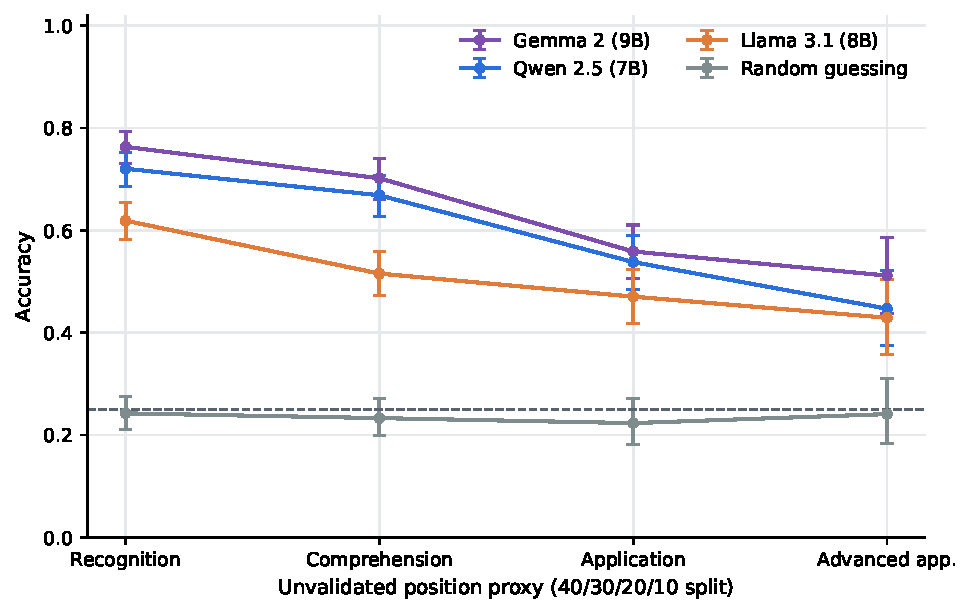
\includegraphics[width=.8\textwidth]{F2_accuracy_by_level.pdf}
\caption{Accuracy by cognitive level (position proxy; 95\% Wilson CI).}\label{fig:level}
\end{figure}

\subsection{Robustness and contamination (RQ3)}
Option shuffling produced the following paired accuracies (Table~\ref{tab:llmshuffle}): Gemma 2 (9B) 67.9\% to 68.6\% ($p=0.513$); Qwen 2.5 (7B) 64.1\% to 65.5\% ($p=0.183$); Llama 3.1 (8B) 53.9\% to 55.3\% ($p=0.279$). The analysis restricted to 1,621 genuinely changed option orders is reported in Table~\ref{tab:shufflechanged}; it excludes the 17 unparseable option sets and 62 identity permutations. Across original-order S1 items, option-letter selection also varied substantially by model (Table~\ref{tab:letters}): against the official key's 29.9\% option A and 23.9\% option C, Llama 3.1 (8B) selected option C on 47.3\% of items and option A on 14.2\%, whereas Qwen 2.5 (7B) (28.5\% A, 22.9\% C) and Gemma 2 (9B) (23.4\% A, 31.2\% C) were closer to balanced. Even a small net accuracy change under shuffling can conceal substantial individual answer flips, shown by the discordant-pair counts in the main table. These tests evaluate option-order sensitivity; they cannot detect all forms of training-data exposure or prove that a model reasons rather than recognises content.

In the audited S2 subset, Qwen 2.5 (7B) was evaluated with brief reasoning in both formats (Tables~\ref{tab:hardresults} and~\ref{tab:hardgap}): chemistry: MCQ 28.1\%, open 15.7\%, gap +12.4 percentage points over 89 pairs ($p=0.043$); physics: MCQ 32.8\%, open 15.5\%, gap +17.2 percentage points over 58 pairs ($p=0.021$). Both science MCQ confidence intervals include the 25\% chance rate, so the format advantages do not imply high absolute competence. On the 89 open-format mathematics items, accuracy was 22.5\% (95\% CI 15.0--32.2\%). Across all 383 S2 responses, 14 final answers were unparseable and 9 reached the output-token limit. A format gap may reflect option elimination, response production, grading constraints or different reasoning demands; it is not a unique signature of memorisation. The year-specific mathematics results (Table~\ref{tab:hardyear}) are based on only 3--21 items per year, with changing item composition, so they do not support a clean training-cut-off test.


\begin{table}[H]\centering\footnotesize
\caption{Accuracy (\%) with original vs shuffled options (paired by item)}\label{tab:llmshuffle}
\begin{tabular}{@{}lrrrrrr@{}}
\toprule
Model & Original & Shuffled & Change & Right$\to$wrong & Wrong$\to$right & McNemar $p$ \\
\midrule
Gemma 2 (9B) & 67.9 & 68.6 & +0.7 & 135 & 147 & 0.513 \\
Qwen 2.5 (7B) & 64.1 & 65.5 & +1.4 & 137 & 161 & 0.183 \\
Llama 3.1 (8B) & 53.9 & 55.3 & +1.4 & 195 & 218 & 0.279 \\
Random guessing & 23.6 & 26.1 & +2.5 & 309 & 351 & 0.110 \\
\bottomrule
\end{tabular}

\end{table}

\subsection{Who gains most from an ``AI answer machine''? (RQ4)}
For Gemma 2 (9B), the average provincial percentile was 93.9 in English and 24.7 in mathematics. Its score lay above the 50th percentile in 100.0\% of English province--year comparisons and 7.4\% of mathematics comparisons; 79.8\% of the English comparisons exceeded the 90th percentile. The correlation between the model's provincial percentile and income was -0.50 in English and -0.44 in mathematics. A fixed model score therefore tends to rank higher against candidates in lower-income provinces in these subjects. This is a descriptive contrast in historical score distributions: it neither measures access to AI nor estimates the causal benefit of AI assistance to an individual candidate.


\section{Discussion}
\paragraph{What the examination rewards} The results show partial, subject-specific automation of past examination content by modest local models. Candidate scores in civic education cluster near the ceiling, so model accuracy must be interpreted against that compressed distribution. English can offer a large relative advantage without near-perfect model accuracy. Linking model scores to contemporaneous candidate distributions therefore changes the policy interpretation of an accuracy-only benchmark. These comparisons describe the historical score scale; rising candidate means cannot be interpreted as improved learning without equating the papers across years.

\paragraph{Security and equity} Local execution demonstrates that answering these items does not require a commercial API or an internet connection during inference. However, a desktop GPU benchmark does not establish performance on a concealed device in an examination room, and neither cheating prevalence nor actual admission advantages are measured here. The provincial gradients indicate where a fixed model score would rank relatively higher, conditional on the historical distributions. They do not imply that poorer candidates have greater access to AI or would gain more from its use. Examination security and equitable access to legitimate learning support should be addressed together, with attention to offline-capable devices and item exposure.

\paragraph{Design implications} Later-position quantitative tasks and the hard numeric subset help locate weaknesses of these model versions, but no item type can be declared permanently AI-resilient. In particular, poor performance on image-dependent items when images were withheld is an input-access limitation, not evidence that modern multimodal AI cannot solve those items. Examination boards should audit complete stimuli with both text and vision models, use new contextualised multi-step tasks, and check whether changing the response format improves the evidence of candidate competence. Our study provides a pre-reform reference for the 2025 changes; it does not evaluate the new true/false or short-answer formats directly. Classroom and performance assessments can complement secure examinations with explicit expectations about permitted AI use \citep{perkins2024aias}.

\paragraph{Responsible item review} These locally deployed models can serve as additional reviewers that flag readily automated items, missing stimuli and option-order sensitivity. This requires secure infrastructure and expert adjudication: a model's failure is not itself evidence of a defective question, and agreement among models does not validate an answer key. The numerical-answer audit in S2 also shows why benchmark construction and grading deserve the same scrutiny as model selection. Repeated evaluations of newly released papers and larger, multimodal models would make this approach more useful for examination design.

\paragraph{Limitations} S1 covers one official paper per subject-year in the pre-2025 format, while S2 is a selected, partly reformulated hard-item subset restricted to decimal answers. The cognitive-level proxy has not been independently validated. Text-only evaluation omits images and the atlas. Results use one deterministic response per condition, one shuffle per item and one reasoning model for S2; they do not measure variation across prompt wording, quantisation or repeated decoding. Output limits and strict numeric parsing can lower measured accuracy. No frontier or multimodal model was tested, and robustness does not rule out training-data exposure. S3 has incomplete coverage in 2017--2019; agreement of national means with official statistics does not establish complete coverage or validate distribution tails. Provincial indicators are cross-sectional (2015, 2018), and ecological associations cannot explain individual inequalities. Percentiles refer to historical candidates who did not necessarily face the same input restrictions as the models. Results describe the specified model versions evaluated in October 2026, rather than the full capability of AI available at that time.

\section{Conclusion}
Three locally deployed open-weight models answered a substantial share of past Vietnamese examination items, with the best overall accuracy reaching 67.9\%, but their candidate-relative advantage varied sharply across subjects. For the best overall model, mean national percentiles were 91.8 in English and 21.4 in mathematics; the corresponding civic-education percentile was 41.1, underscoring the need to interpret accuracy against each subject's candidate distribution. Option-order and response-format experiments identify behavioural sensitivity without establishing contamination, while provincial analyses show that a common model score can imply different relative positions across income contexts. Examination reform should combine secure administration with repeated audits using complete stimuli, newly released items and transparent grading, rather than treating any format as permanently AI-resilient.


\section*{Data and code availability}\label{sec:availability}
All five source repositories are publicly accessible (Table~\ref{tab:sources}). The local reproducibility package contains download and analysis scripts, prompts, raw model outputs, the continuation model manifest and exclusion logs. A persistent public release of this package has not yet been deposited. Individual candidate records are analysed only in aggregate and are not redistributed. The candidate-score repository is a third-party mirror; its account identifier is recorded for provenance without assigning an unverified personal identity or attributing this mirror to MOET.

\section*{Declaration of generative AI use}
LLMs are the object of study. OpenAI Codex was also used to assist with code review, the local experiment workflow, numerical-grading checks, manuscript drafting and LaTeX editing. The authors must review the resulting code, analyses and text and take responsibility for the submitted manuscript.

\ifdefined\APASeven
  \printbibliography
\else
  \bibliographystyle{apacite}
  \bibliography{refs}
\fi

\appendix
\renewcommand{\theHtable}{\Alph{section}.\arabic{table}}
\section{Validation of candidate-level scores}
\setcounter{table}{0}
\begin{table}[H]\centering\footnotesize
\caption{National means from S3 vs MOET published means}\label{tab:validation}
\begin{tabular}{@{}lrrrrr@{}}
\toprule
Subject & Year & MOET & S3 & Difference & $N$ (S3) \\
\midrule
Mathematics & 2019 & 5.64 & 5.57 & -0.07 & 807,762 \\
Physics & 2019 & 5.57 & 5.56 & -0.01 & 292,166 \\
Chemistry & 2019 & 5.35 & 5.34 & -0.01 & 295,544 \\
Biology & 2019 & 4.68 & 4.67 & -0.01 & 291,199 \\
History & 2019 & 4.30 & 4.29 & -0.01 & 542,729 \\
Geography & 2019 & 6.00 & 5.99 & -0.01 & 535,897 \\
Civic education & 2019 & 7.37 & 7.35 & -0.02 & 470,905 \\
English & 2019 & 4.36 & 4.24 & -0.12 & 728,513 \\
Mathematics & 2020 & 6.68 & 6.66 & -0.02 & 866,581 \\
Physics & 2020 & 6.72 & 6.72 & -0.00 & 293,287 \\
Chemistry & 2020 & 6.71 & 6.71 & -0.01 & 295,536 \\
Biology & 2020 & 5.59 & 5.59 & -0.00 & 290,377 \\
History & 2020 & 5.19 & 5.18 & -0.01 & 568,581 \\
Geography & 2020 & 6.78 & 6.77 & -0.01 & 555,072 \\
Civic education & 2020 & 8.14 & 8.12 & -0.01 & 482,980 \\
English & 2020 & 4.58 & 4.57 & -0.01 & 772,098 \\
Mathematics & 2021 & 6.61 & 6.62 & +0.01 & 924,651 \\
Mathematics & 2022 & 6.47 & 6.47 & -0.00 & 982,670 \\
Biology & 2022 & 5.02 & 5.02 & -0.00 & 322,185 \\
History & 2022 & 6.34 & 6.34 & +0.00 & 659,617 \\
English & 2022 & 5.15 & 5.16 & +0.01 & 870,571 \\
Mathematics & 2023 & 6.25 & 6.25 & +0.00 & 1,003,373 \\
Physics & 2023 & 6.57 & 6.57 & +0.00 & 327,189 \\
Chemistry & 2023 & 6.74 & 6.75 & +0.01 & 328,118 \\
Biology & 2023 & 6.39 & 6.39 & +0.01 & 324,625 \\
History & 2023 & 6.03 & 6.03 & -0.00 & 683,447 \\
Geography & 2023 & 6.15 & 6.15 & -0.00 & 682,134 \\
Civic education & 2023 & 8.29 & 8.29 & -0.00 & 565,452 \\
English & 2023 & 5.45 & 5.46 & +0.01 & 880,997 \\
\bottomrule
\end{tabular}

\end{table}

\section{Hard-item response-format results}
\setcounter{table}{0}
\begin{table}[H]\centering\footnotesize
\caption{Qwen2.5-7B with brief reasoning on audited S2 items; 95\% Wilson intervals (\%)}\label{tab:hardresults}
\begin{tabular}{@{}llrrrr@{}}
\toprule
Model / subject & Format & $N$ & Accuracy (\%) & Lower CI & Upper CI \\
\midrule
Qwen 2.5 (7B) (CoT) / Chemistry & MCQ & 89 & 28.1 & 19.8 & 38.2 \\
Qwen 2.5 (7B) (CoT) / Chemistry & OPEN & 89 & 15.7 & 9.6 & 24.7 \\
Qwen 2.5 (7B) (CoT) / Mathematics & OPEN & 89 & 22.5 & 15.0 & 32.2 \\
Qwen 2.5 (7B) (CoT) / Physics & MCQ & 58 & 32.8 & 22.1 & 45.6 \\
Qwen 2.5 (7B) (CoT) / Physics & OPEN & 58 & 15.5 & 8.4 & 26.9 \\
\bottomrule
\end{tabular}

\end{table}

\begin{table}[H]\centering\footnotesize
\caption{Paired MCQ--open contrasts for Qwen2.5-7B; McNemar exact tests}\label{tab:hardgap}
\begin{tabular}{@{}lrrrrrr@{}}
\toprule
Subject & Pairs & MCQ (\%) & Open (\%) & Gap (pp) & \makecell{MCQ only /\\open only} & $p$ \\
\midrule
Chemistry & 89 & 28.1 & 15.7 & +12.4 & 18 / 7 & 0.0433 \\
Physics & 58 & 32.8 & 15.5 & +17.2 & 13 / 3 & 0.0213 \\
\bottomrule
\end{tabular}

\end{table}

\begin{table}[H]\centering\footnotesize
\caption{Qwen2.5-7B open-format mathematics accuracy by recorded paper year; 95\% Wilson intervals (\%)}\label{tab:hardyear}
\begin{tabular}{@{}rrrrr@{}}
\toprule
Year & $N$ & Accuracy (\%) & Lower CI & Upper CI \\
\midrule
2017 & 18 & 33.3 & 16.3 & 56.3 \\
2018 & 15 & 20.0 & 7.0 & 45.2 \\
2019 & 6 & 0.0 & 0.0 & 39.0 \\
2020 & 16 & 56.2 & 33.2 & 76.9 \\
2021 & 21 & 9.5 & 2.7 & 28.9 \\
2022 & 3 & 0.0 & 0.0 & 56.1 \\
2023 & 6 & 0.0 & 0.0 & 39.0 \\
2024 & 4 & 0.0 & 0.0 & 49.0 \\
\bottomrule
\end{tabular}

\end{table}

\section{Option-order sensitivity on changed presentations}
\setcounter{table}{0}
\begin{table}[H]\centering\footnotesize
\caption{Option-order comparison restricted to 1,621 items whose order actually changed (17 unparseable option sets and 62 identity permutations excluded)}\label{tab:shufflechanged}
\begin{tabular}{@{}lrrrrr@{}}
\toprule
Model & Pairs & Original (\%) & Shuffled (\%) & Change (pp) & $p$ \\
\midrule
Gemma 2 (9B) & 1621 & 67.4 & 68.2 & +0.7 & 0.513 \\
Qwen 2.5 (7B) & 1621 & 64.0 & 65.5 & +1.5 & 0.181 \\
Llama 3.1 (8B) & 1621 & 53.6 & 54.9 & +1.3 & 0.323 \\
Random guessing & 1621 & 23.4 & 26.0 & +2.6 & 0.110 \\
\bottomrule
\end{tabular}

\end{table}

\section{Candidate-coverage sensitivity}
\setcounter{table}{0}
National percentile summaries were recalculated after excluding 2019, the only S1 paper year with documented incomplete candidate coverage. For Gemma 2 (9B), English changes from 91.8 to 90.5 and mathematics from 21.4 to 24.8. The strong subject contrast persists; across the three models and eight subjects, changes range from $-7.6$ to $+7.2$ percentage points. This is a different-year sensitivity analysis, not a correction of the missing 2019 candidates: paper difficulty and cohort composition also change. The incomplete 2017--2018 data still affect the descriptive eight-year trends.
\begin{table}[H]\centering\footnotesize
\caption{Mean national percentiles including and excluding the incomplete 2019 candidate cohort}\label{tab:coverage}
\begin{tabular}{@{}llrrr@{}}
\toprule
Model & Subject & 2019--2023 & 2020--2023 & Difference (pp) \\
\midrule
Gemma 2 (9B) & Biology & 85.5 & 82.8 & -2.6 \\
Gemma 2 (9B) & Chemistry & 39.3 & 35.8 & -3.5 \\
Gemma 2 (9B) & Civic education & 41.1 & 43.4 & +2.3 \\
Gemma 2 (9B) & English & 91.8 & 90.5 & -1.3 \\
Gemma 2 (9B) & Geography & 33.5 & 36.1 & +2.6 \\
Gemma 2 (9B) & History & 81.9 & 78.1 & -3.8 \\
Gemma 2 (9B) & Mathematics & 21.4 & 24.8 & +3.3 \\
Gemma 2 (9B) & Physics & 32.5 & 27.2 & -5.3 \\
Llama 3.1 (8B) & Biology & 34.1 & 37.8 & +3.7 \\
Llama 3.1 (8B) & Chemistry & 19.2 & 16.8 & -2.4 \\
Llama 3.1 (8B) & Civic education & 32.5 & 30.9 & -1.6 \\
Llama 3.1 (8B) & English & 73.3 & 69.7 & -3.6 \\
Llama 3.1 (8B) & Geography & 33.1 & 37.0 & +3.9 \\
Llama 3.1 (8B) & History & 64.6 & 71.9 & +7.2 \\
Llama 3.1 (8B) & Mathematics & 4.5 & 3.6 & -0.9 \\
Llama 3.1 (8B) & Physics & 9.7 & 10.0 & +0.3 \\
Qwen 2.5 (7B) & Biology & 61.2 & 53.5 & -7.6 \\
Qwen 2.5 (7B) & Chemistry & 27.1 & 25.5 & -1.6 \\
Qwen 2.5 (7B) & Civic education & 30.3 & 29.9 & -0.4 \\
Qwen 2.5 (7B) & English & 91.5 & 90.3 & -1.2 \\
Qwen 2.5 (7B) & Geography & 45.4 & 49.3 & +4.0 \\
Qwen 2.5 (7B) & History & 74.9 & 72.8 & -2.1 \\
Qwen 2.5 (7B) & Mathematics & 22.3 & 24.2 & +1.9 \\
Qwen 2.5 (7B) & Physics & 22.4 & 20.8 & -1.5 \\
\bottomrule
\end{tabular}

\end{table}

\end{document}

